\section{Technical Description}

\label{sec:technical_description}

\subsection{Background}
\label{subsec:technical:background}
As mentioned, this design is heavily based on the Long Wavelength Array antenna element design.
The reader is highly encouraged to review the relevant documents from the LWA Memo Series as full description of their design is outside the scope of this document \cite{lwa_memo}.
Table \ref{table:lwa_relevant_docs} below gives a list of the key documents from the LWA Memo Series used in this work.
However, when necessary, details of the LWA design will be discussed, particularly when discussing deviations from the LWA design as summarized in Table \ref{table:lwa_differences}.
The documents listed in the table pertain specifically to the technical design of the active balun board.
There are a number of other documents on the LWA Memo Series \cite{lwa_memo} that discuss topics such as the antenna element design (blade, wire, etc.), antenna patterns, ground screens, RFI site surveys, potential applications of the LWA, along with many other topics for the overall radio observatory that are not relevant to this work (though all make for very interesting reads).

\begin{table}[h]
\begin{center}
\caption{Relevant documents from the LWA Memo Series.}
\label{table:lwa_relevant_docs}
\begin{tabular}{|c|p{15cm}|}
	\hline
	\textbf{Memo\#} & \textbf{Document Title} \\
	\hline
	190 & Collected LWA Engineering Memos from the Development of the Front End Electronics (FEE) \cite{lwa_memo_190} \\
	\hline
    188 & Preliminary Design of the LWA-1 Array, Antenna, Stand, Front End Electronics, and Ground Screen \cite{lwa_memo_188} \\
	\hline
	87 & A Comparison of Two Power Combining Elements for LWA Active-Baluns -  180$^{\circ}$  Hybrid versus Wideband Transformer \cite{lwa_memo_87}\\
	\hline
	120 & The Rapid Test Array Balun (G250R) \cite{lwa_memo_120} \\
	\hline
	135 & Bias-T Design Considerations for the LWA \cite{lwa_memo_135}\\
	\hline
\end{tabular}
\end{center}
\end{table}

\subsection{Design Feature Overview}
\label{subsec:technical:overview}
A single balun board provides the necessary electronics for a single linearly polarized HF dipole antenna.
The active balun board provides good performance across the objective frequency of operation from approximately 1.5 to 50.0 MHz, with good rejection in the AM and FM broadcast bands.
The performance values given in this section are the average values for the nominal frequency of operation, with more detailed measured performance given in later sections.
The active balun board provides an average gain of 36.1 dB.
The input third order intercept point (IIP3) is approximately -2.5 to -3.0 dBm across the operating band.
The input 1dB Compression Point (P1dB) is approximately -18.41 dBm across the operating band.
Note that linearity measurements (IIP3 and P1dB) are taken with the output ESD protection diodes removed from the boards under test, per the measurement techniques described in the LWA documents.

The active HF dipole balun board utilizes a pair of GALI-74+ amplifiers from Mini-Circuits as the primary active amplifier device, one for each element of a single dipole.
The signals from each dipole element are then combined using the secondary coil of a Mini-Circuits ADT2-1T RF transformer, which also provides a 180 degree phase shift between the two elements.
The ADT2-1T transformer also provides a 2:1 impedance ratio, converting a nominal 100$\Omega$ secondary coil to a 50$\Omega$ output impedance on the primary coil.
The signal is then routed through either a low pass or a band pass RFI filter via surface mount solder jumpers.
In its default configuration, these filters are bypassed with a surface mount trace that can be cut with a razor blade if the the filters are desired to be used.
The output of the filters are then passed to a GALI-6 amplifier.

A number of surge protection devices and decisions are included in the LWA-FEEv1.7 design and remain essentially unaltered in this design. 
This includes 1N914 double backed diodes on the RF input and RF output lines serving as ESD protection.
The design also includes a Gas Discharge tube on the RF output path to protect back end electronics from damaging lightning surges.
These diodes directly effect the measurement process, particularly with respect to linearity measurements (IIP3 and P1dB), as mentioned previously.
Finally, the two input capacitors, connected to the dipole element arms, are rated for 1000 volts.  
This decision is elaborated on in the failure analyses presented in the LWA documentation \cite{lwa_memo_190} where the original capacitors had failed short.
This was presumably due to nearby lighting that produced an overvoltage condition. 

The PCB hole patterns are designed so that a second balun board can be flipped 180 degrees along the top left to bottom right diagonal and maintain proper alignment.
When this is done, the two boards can be mechanically mated and held together with four 4-40 screws.
The solder mask on the bottom of the PCBs has been removed such that the ground planes of the two boards are also electrically connected.
The second PCB SMA connector can then be mounted on the bottom of the PCB and aligned with the large hole in the upper right section of the top PCB, resulting in both SMA connectors pointing `up.`

Each balun board consumes approximately 250 mA when supplied with approximately 13.8VDC.
Power is nominally supplied via the output RF coaxial cable, and the design contains an integrated bias-t circuit.
In addition, the board allows for direct supply of power via solder pads that bypass the input bias-t.
The bias-t can be completely disconnected from the output RF by disconnecting a solder jumper, though the expected power arrangement when fielded should be via the coaxial cable, which provides a degree of shielding, rather than via a separate power line (which also increases overall costs).

\begin{table}[h!]
\begin{center}
\caption{Summary of Active HF Dipole Balun Performance Parameters.}
\label{table:ahfdb_features}
\begin{tabular}{|l|l|l|l|}
	\hline
	\textbf{Parameter} & \textbf{Symbol} & \textbf{Unit} & \textbf{Value}\\
	\hline
	Frequency of Operation & $f_{nom}$  & MHz & 1.5 to 50 \\
	\hline
	Integrated BPF, low -3dB cutoff & $f_{lo}$ & MHz & 1.0 \\
	\hline
	Integrated BPF, high -3dB cutoff & $f_{hi}$ & MHz & 50.0 \\
	\hline
	Integrated BPF, high -3dB cutoff & $f_{hi}$ & MHz & 50.0 \\
	\hline
	Average Gain & $G_{avg}$ & dB & 36.1\\
	\hline
	Input Compression Point & $P1dB$ & dBm & -18.41 \\
	\hline
	Input Third Order Intercept Point & $IIP3$ & dBm & -2.5 to -3.0 \\
	\hline
	DC Input Voltage, Range & $V_{in,range}$ & V & 10.0 to 35.0 \\
	\hline
	DC Input Voltage, Nominal & $V_{in,nom}$ & V & 13.8 \\
	\hline
	DC Supply Current, Nominal & $I_{supply}$ & mA & 250.0 \\
	\hline
	DC Supply Method, Nominal & N/A & N/A & bias-t via coax \\
	\hline
	DC Supply Method, Alternate & N/A & N/A & external \\
	\hline	
	
\end{tabular}
\end{center}
\end{table}



\subsection{Design Deviations from LWA}
\label{subsec:technical:deviation}

\begin{table}[h!]
\begin{center}
\caption{Summary of design deviations from the LWA-FEEv1.7 reference design.}
\label{table:lwa_differences}
\begin{tabular}{|l|l|}
	\hline
	\textbf{LWA Design} & \textbf{AHFDB Design} \\
	\hline
	Frequency: 10 to 88 MHz & Frequency: 1.5 to 50 MHz\\
	\hline
	Teletech 180$^{\circ}$ hybrid combiner & Mini-Circuits RF transformer\\
	\hline
	Low Pass Filter & LPF, BPF, Filter Bypass\\
	\hline
	12V Voltage Regulator & 8V Voltage Regulator \\
	\hline
	LWA-FEEv1.7 PCB form factor & More compact PCB form factor\\
	\hline
\end{tabular}
\end{center}
\end{table}

\subsubsection{180$^{\circ}$ Hybrid Combiner vs RF Transformer}
\label{subsubsec:technical:deviation:hybrid}
The LWA-FEEv1.7 utilizes a Tele-Tech HX62A 180$^{\circ}$ hybrid combiner to combine the signals from each side of a single polarization dipole element.
The LWA documentation quotes various costs for this single component range from \$20.00 per unit when $>$500 are purchased \cite{lwa_memo_188} to \$31.50 per unit $>$500 units are purchased \cite{lwa_memo_190}.
The lower cost is from a more recent document (2009), and for a dual polarization implementation two of these units would be required.
The cost for 2 units is likely higher than the quoted costs which assumes a purchase quantity of more than 500 units.
This is cost prohibitive for this project, therefore it was decided that the Tele-Tech HX62A is a non-starter for this project and a suitable, lower cost alternative is required, even if that means accepting a compromise in performance.

The LWA engineers performed an analysis comparing the Tele-Tech HX62A to a Mini-Circuits ADT2-2-1T-1P RF transformer \cite{lwa_memo_87}.
The results of the analysis show that the HX62A outperforms the ADT2-2-1T-1P.
The conclusion of that document is that the increased cost of the Tele-Tech device is worth the increased performance for the LWA design goals.
The Mini-Circuits component is drastically lower in cost, and the author believed it was a suitable for this project.
However, according to the Mini-Circuits ADT2-2-1T-1P datasheet, the low end frequency response bottoms out around 8 MHz, and the new design is striving for low end performance down to approximately 1.5 MHz to cover the 160m Amateur Radio Band.
Alternatively, the Mini-Circuits ADT2-1T datasheet shows a low end response of 0.4 MHz, as well as decreased insertion loss and better return loss across the HF band.
The cost of this device is \$5.77 per unit on Minicircuits.
For this reason, the ADT2-1T was selected for this project.

\begin{table}[h!]
\begin{center}
\caption{Pinouts of the Mini-Circuits ADT2-2-1T-1P \& the ADT2-1T RF transformers}
\label{table:rf_transformer_pinout}
\begin{tabular}{|c|l|l|}
	\hline
	\textbf{Pin} & \textbf{ADT2-2-1T-1P} & \textbf{ADT2-1T} \\
	\hline
	1 & primary & primary \\
	\hline
	2 & not used & not used \\
	\hline
	3 & primary dot & primary dot \\
	\hline
	4 & secondary dot & secondary \\
	\hline
	5 & secondary ct & secondary ct\\
	\hline
	6 & secondary & secondary dot\\
	\hline
\end{tabular}
\end{center}
\end{table}

Table \ref{table:rf_transformer_pinout} shows the pinouts for the RF transformers.
Careful scrutiny of pins 4 and 6 shows that there is an inversion of the secondary between the two transformers, which has implications for the phase of the output signal on the primary coil.
In the LWA comparison document \cite{lwa_memo_87}, pin 3 (primary dot signal) is grounded.
Due to the inversion of the primary/secondary orientation on the ADT2-1T compared to the ADT2-2-1-T, the author elected to include solder jumpers in the PCB layout that allows alternate signal routing paths.
This allows for experimentation with which pin is grounded and the resulting phase.
For the default test case in the version 1, rev- design, pin 1 (primary signal) is grounded to account for the phase inversion.
Likely, this concern probably doesn't matter as long as the active balun boards are consistent, therefore the solder jumpers will likely be removed in future revisions.

\subsubsection{Filtering}
\label{subsubsec:technical:deviation:filtering}
The original LWA design utilizes a 5 pole Butterworth Low Pass Filter (LPF) as a modest Radio Frequency Interference (RFI) filter with a -3dB cutoff frequency of approximately 150 MHz.
Figure \ref{fig:lwa_lpf} below shows a Quiet Universal Circuit Simulator (QUCS) simulation of the LWA LPF included in the LWA-FEEv1.7 according to the LWA design documents \cite{lwa_memo_190}.
With a 3dB bandwidth that spans DC to 150 MHz, effectively no rejection of either the broadcast AM or broadcast FM bands are provided.

\begin{figure}[h!]
  \centering
  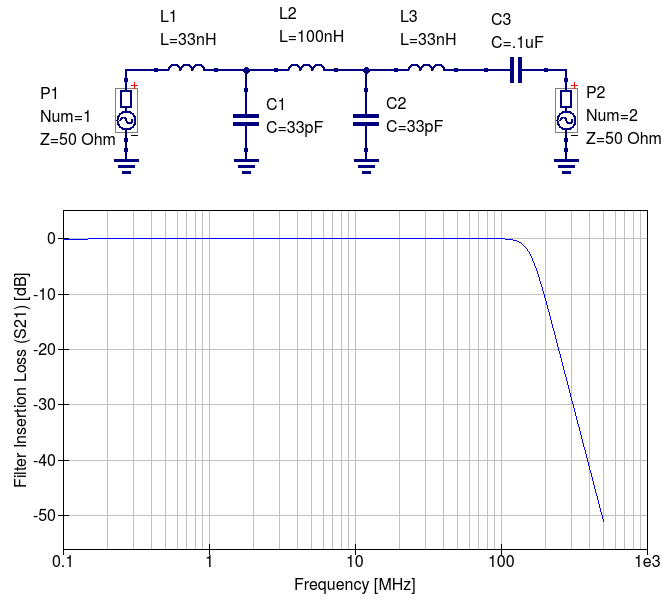
\includegraphics[width=0.55\linewidth]{figures/lwa_lpf.png}
  \caption{LWA-FEEv1.7 low pass filter schematic and response simulation in QUCS.}
  \label{fig:lwa_lpf}
\end{figure}

As described earlier, a design goal of this project is to aim for a nominal operating bandwidth between 1.5 MHz and 50.0 MHz.
Another goal is to provide some amount of rejection to the broadcast AM and broadcast FM bands.
While some of the LWA documents do discuss the inclusion of a notch filter for the broadcast FM band around 98 MHz (center of the FM band), due to the overall changes in the desired operating frequency, the author elected to replace the LPF with a bandpass filter (BPF).
For experimentation purposes, the author elected to also include a low pass filter with a modified -3dB cutoff frequency of 50 MHz.
Again, selection of the desired filter (LPF or BPF) is accomplished via solder jumper signal routing.
In addition to the LPF and BPF, the actual default configuration of the filter section of the PCB is to bypass all filters, again with a surface mount PCB jumper.
During initial PCB assembly, this jumper can be cut with a small razor blade and the solder jumpers are then used to route the signal through either the BPF or the LPF. 
The author utilized QUCS to design the initial filters, which are 5 both pole Butterworth designs.
The computed ideal values for the capacitors and inductors were then modified to match readily available standard values.
The circuit design and results of the QUCS simulation for the new LPF is shown in Figure \ref{fig:ahfdb_filter:lpf} and for the new BPF in Figure \ref{fig:ahfdb_filter:bpf}.

\begin{figure}[h]
  \centering
  \begin{subfigure}{.48\textwidth}
    \centering
    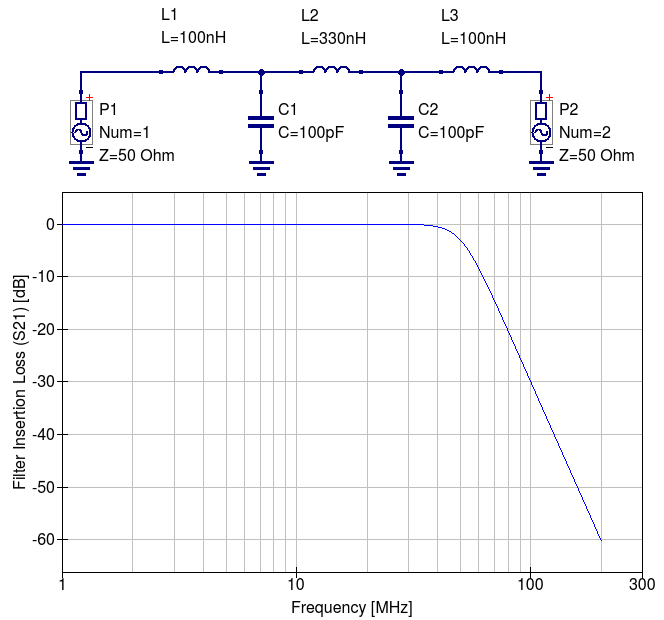
\includegraphics[width=.93\linewidth]{figures/lwa_lpf_50MHz.png}
    \caption{AHFDB v1,rev- low pass filter.}
	\label{fig:ahfdb_filter:lpf}
  \end{subfigure}%
  \begin{subfigure}{.48\textwidth}
    \centering
    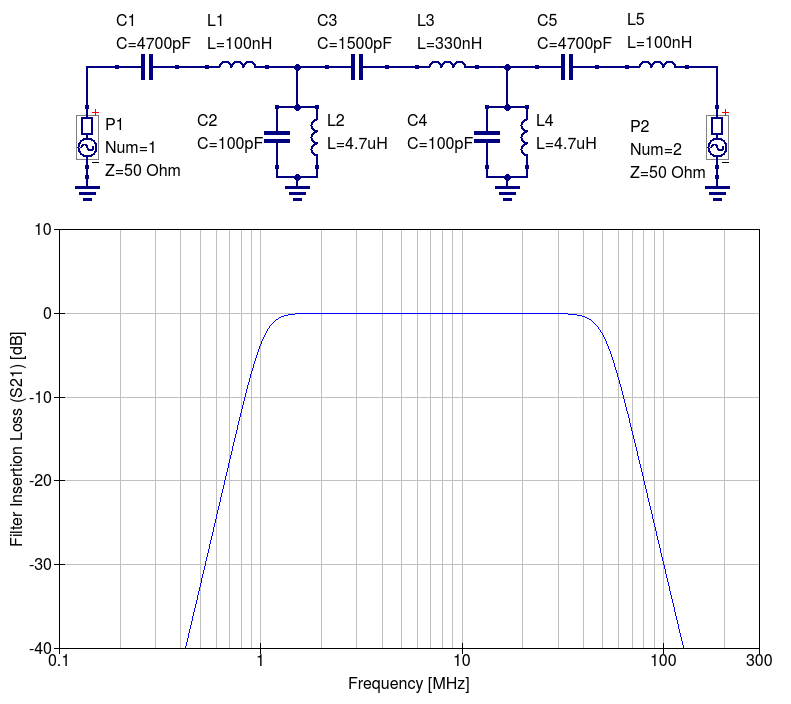
\includegraphics[width=\linewidth]{figures/lwa_bpf_1MHz_50MHz.png}
    \caption{AHFDB v1,rev- band pass filter.}
	\label{fig:ahfdb_filter:bpf}
  \end{subfigure}
  \caption{Active HF dipole balun version 1, revision- (AHFDB, v1, rev-) low pass filter schematic and response simulation in QUCS.}
  \label{fig:ahfdb_filter}
\end{figure}

Notice the upper -3dB cutoff frequency for both filters in Figure \ref{fig:ahfdb_filter} is approximately 50 MHz.
At approximately 98 MHz, the center of the broadcast FM band, both filters achieve approximately -30 dB of rejection.
The lower -3dB cutoff frequency of the BPF is approximately 1.0 MHz, with minimal insertion loss around 1.8 MHz (the low end of the Amateur Radio 160m band).
This low end is a bit below the upper edge of the AM broadcast band (1.6 MHz), but because of the close proximity to the Amateur Radio 160m band, a balance had to be struck.
For this first test, it was decided to go with the 1 MHz cutoff as the actual filter performance is not expected to perfectly match the QUCS simulations and the design could be optimized later.
On air performance tests at the author's QTH, presented in more detail later, shows this provides sufficient AM band rejection of local nearby AM stations (including one station less than 1 mile from the author's QTH).
Adding additional poles to the filters is possible, but will increase insertion loss in the pass band.
Adding a notch filter is also feasible.
As this is an Open Hardware design, including the QUCS simulations, KiCAD schematic, and PCB layout, others are encouraged to experiment with these values to find the right filter response for their local RFI environment.

\subsubsection{Voltage Regulator}
\label{subsubsec:technical:deviation:vreg}
The LWA-FEEv1.7 utilizes a 12V voltage regulator onboard the PCB.
For this design, the author has considered the possibility that the antenna may be utilized during portable operations operating from batteries.
Prior experience has shown that nominal 12V batteries when fully charged can reach voltages in excess of 14 volts.
When depleted 12V batteries can drop as low as 10 to 11 Volts.
Therefore, the author made a design decision to down size the onboard voltage regulator to an 8 volt output voltage regulator in order to allow operation at supply voltages as low as approximately 10 volts.
This decision has a couple of implications.

First, the bias resistors for the GALI-74 and GALI-6 amplifiers must be modified to account for this change in the overall supply voltage.
This is easily accomplished and the Mini-Circuits datasheets provide recommended bias resistor values for various circuit supply voltages.
The author did actually experiment with lower than recommended bias resistor values in order to increase the current draw of the balun boards.
This was done based on the higher compression point and third order intercept point values shown in the detailed test data documents provided by Mini-Circuits.
Ultimately though, this was abandoned and the author reverted to a single bias resistor value of 39 ohms for all three RF amplifiers in the design.
Further linearity testing may be conducted on future revisions of the design.

Second, a single polarization board pull approximately 250 mA (at 13.8V input voltage).
When using a standard 13.8V power supply (common in Amateur Radio), this results in a voltage difference of approximately 5.8V between the input and output voltages of the regulator.
A simple rule of thumb for computing the waste power through a linear regulator is to multiply the current draw by the voltage difference.
This results in approximately 1.45 Watts of waste power for a single board and approximately 2.90 Watts when configured for dual polarization. 
This waste power is not insignificant and manifests in the form of heat.
The voltage regulator is a D2PAK form factor and the heat is conducted into the ground plane of the PCB.
The ground planes of a dual polarization stack are in contact with each other when mechanically mated.
The result of all this is that the temperature of the balun boards achieved a fairly high temperature that was hot to the touch.
However, no part of the board was hot enough to cause burns or pain and the increased temperature may actually help stabilize the overall balun temperature when fielded in a completed system, particularly in colder regions.

\subsection{Polarization}
A single active balun PCB board provides a single linearly polarized, electrically small dipole, also referred to as a short dipole.
The PCB is designed in such a way that a pair of active balun boards can be stacked together to produce a crossed dipole.
The crossed dipole design is desirable in order to discriminate between Ordinary and Extraordinary mode waves.  
Like the LWA, the author intends to explore the use of digital receiver techniques for digitizing each linear element.
The combining of the signals to produce any polarization, from linear, to elliptical, to circular can then be done in software (i.e. GNU Radio) to explore measurement techniques of the propagating wave Stokes parameters.
Alternatively, experimenters may employ a 90 degree hybrid to directly produce Right Hand Circular Polarization (RHCP) and Left Hand Circular Polarization (LHCP) in the analog domain (refer to the Reeve observatory site for more information on this topic \cite{reeve_observatory}).



Ordinary and Extraordinary discrimination (RHCP/LHCP)



\begin{figure}[h]
  \centering
  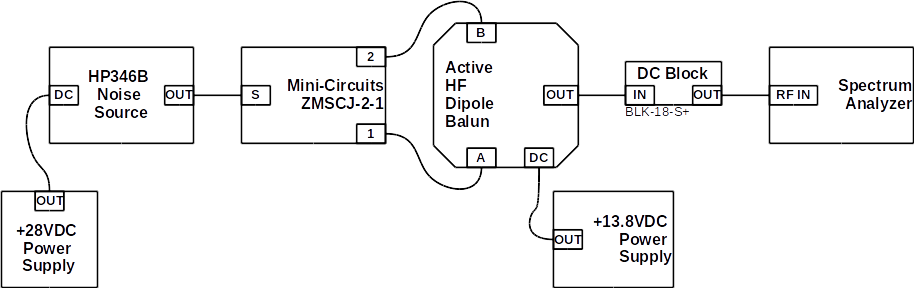
\includegraphics[width=0.8\linewidth]{figures/noise_figure.png}
  \caption{Noise Figure Measurement Setup.}
  \label{fig:noise_figure}
\end{figure}




